\documentclass[fleqn,10pt]{wlscirep}
\usepackage[T1]{fontenc}
\usepackage[utf8]{inputenc}
\usepackage{mathptmx}
\usepackage{booktabs,dcolumn}
\usepackage{color, colortbl}
\usepackage{graphicx}
\usepackage{hyperref}
\definecolor{Blue}{rgb}{0.31, 0.51, 0.75}
\definecolor{LightBlue}{rgb}{0.81, 0.85, 0.91}

\bibliographystyle{naturemag-doi}

\title{Identification of Long Non-Coding RNA Signatures for Diagnosis and Prognosis of Colorectal Cancer via Machine Learning}

\author[1]{Zhuha Zhou}
\author[1]{Yongyu Bai}
\author[2]{Qigang Xue}
\author[3]{Zhuxian Zhou}
\author[1*]{Shaolian Han}
\affil[1]{Department of Gastroenterology Surgery, The First Affiliated Hospital of Wenzhou Medical University, Nanbaixiang Street, Ouhai District, 325000, Wenzhou, Zhejiang, China.}
\affil[2]{Department of Hepatobiliary and Pancreatic Surgery, The First Affiliated Hospital of Wenzhou Medical University, Nanbaixiang Street, Ouhai District, 325000, Wenzhou, Zhejiang, China.}
\affil[3]{Center for Bionanoengineering and Key Laboratory of Biomass Chemical Engineering of Ministry of Education, College of Chemical and Biological Engineering, Zhejiang University, Zheda Road 38, 310027, Hangzhou, China.}
\affil[*]{Correspondence and requests for materials should be addressed to S.H. (email: wangguanyu@zju.edu.cn)}

\begin{abstract}
Colorectal cancer (CRC) remains a leading cause of cancer-related mortality, yet clinically actionable molecular biomarkers for early detection and prognosis are still limited. Long non-coding RNAs (lncRNAs) have emerged as promising biomarkers, but identifying robust signatures from high-dimensional transcriptomic data requires systematic computational strategies. Here, we integrate differential expression analysis with elastic-net regularized Cox regression and five machine learning classifiers to discover lncRNA signatures with both diagnostic and prognostic value in CRC. Using the TOIL-recomputed TCGA--GTEx dataset (349 non-tumor, 290 tumor samples) and TCGA-COAD clinical follow-up data (428 patients), we identified 17 candidate lncRNAs via elastic-net Cox regression ($\alpha = 0.200$, $\lambda = 0.230$) and further refined them to an 8-lncRNA panel through stepwise multivariate Cox regression (AIC = 615.76, C-index = 0.82). The resulting risk score model stratified patients into distinct prognostic groups (log-rank $p < 0.0001$ in the training set; $p = 0.0028$ in the testing set), with time-dependent AUC converging to 0.725 at 8 years. Among classification models, support vector machine (SVM), random forest, and neural network achieved testing-set accuracies of 92.1\%, 91.1\%, and 92.1\%, respectively (AUC 0.969--0.974), substantially outperforming logistic regression (64.9\%) and elastic-net logistic regression (64.4\%). Notably, our top-ranked lncRNA MIR210HG (HR = 1.40, $p = 0.0003$) is an established oncogenic transcript that inhibits ferroptosis in colon cancer via the PCBP1 axis, while several high-ranking lncRNAs (CTB-25B13.12, AP006621.5, RP11-549B18.1) represent novel candidates with no prior functional characterization. Our findings demonstrate that machine learning-driven analysis of lncRNA expression profiles can yield clinically relevant diagnostic and prognostic biomarkers for CRC, and we provide a fully reproducible computational pipeline for future biomarker discovery studies.
\end{abstract}

\noindent\textbf{Keywords:} colorectal cancer, long non-coding RNA, machine learning, biomarker, diagnosis, prognosis, Cox proportional hazards, elastic net, MIR210HG

\begin{document}
\flushbottom
\maketitle
\thispagestyle{empty}

\section*{Introduction}

Colorectal cancer (CRC) is the third most frequently diagnosed malignancy and the second leading cause of cancer-associated death worldwide, accounting for approximately 1.9 million new cases and 900,000 deaths annually\cite{RN1}. Despite advances in screening and treatment, the majority of CRC cases are diagnosed at advanced stages, when lymph node involvement or distant metastasis has already occurred. The 5-year survival rates decline sharply from 91.1\% for localized disease to 69.8\% for regional spread and 11\% for distant metastasis, underscoring the urgent need for molecular biomarkers that enable early detection and accurate prognostication\cite{RN1,RN2}.

Long non-coding RNAs (lncRNAs) are transcripts longer than 200 nucleotides that do not encode proteins but function as versatile regulators of gene expression at epigenetic, transcriptional, and post-transcriptional levels\cite{RN3}. Accumulating evidence demonstrates that lncRNAs participate in cancer hallmarks including proliferation, invasion, metastasis, and drug resistance, and several lncRNAs have been specifically implicated in CRC pathogenesis through diverse molecular mechanisms\cite{RN4,RN5,RN6}. Because lncRNAs exhibit tissue-specific and disease-specific expression patterns, they are increasingly recognized as promising biomarkers and therapeutic targets for clinical applications\cite{RN7,RN8,RN9}. However, traditional experimental approaches for discovering disease-associated lncRNAs are time-consuming and low-throughput, creating a strong incentive for computational methods that can systematically prioritize candidates from large-scale sequencing data.

The public availability of RNA-sequencing datasets from The Cancer Genome Atlas (TCGA)\cite{RN10} and the Genotype-Tissue Expression (GTEx)\cite{RN11} projects has created unprecedented opportunities for transcriptome-wide biomarker discovery. Notably, the TOIL project at the University of California, Santa Cruz, has recomputed TCGA and GTEx raw expression data through a unified pipeline, minimizing batch effects and enabling direct comparison between tumor and normal tissues\cite{RN12}. This harmonized resource provides a statistically well-powered foundation for identifying differentially expressed lncRNAs, particularly because the original TCGA-COAD cohort contains only 41 adjacent non-tumor samples, which is insufficient for robust differential expression analysis.

Machine learning has emerged as a transformative tool in oncology research, with applications spanning histopathological diagnosis, radiomics-based prognostication, and genomic biomarker discovery\cite{RN13}. Supervised classification algorithms can distinguish cancerous from normal tissues with high accuracy, while survival models estimate patient risk over time\cite{RN14,RN15}. Despite these advances, the application of machine learning to lncRNA-based biomarker discovery remains relatively underexplored. The \texttt{caret} package in R provides a unified interface that streamlines model training, hyperparameter tuning, and performance evaluation across diverse algorithms\cite{RN16}. Zhang \textit{et al.} developed CRlncRC, a machine learning-based classifier for cancer-related lncRNAs integrating multiple optimization strategies\cite{RN17}. However, studies that simultaneously assess diagnostic and prognostic utility of lncRNA signatures using standardized, reproducible machine learning pipelines remain scarce\cite{RN18,RN19}.

In this study, we designed an integrated computational pipeline to identify lncRNA signatures with dual diagnostic and prognostic value in CRC. Our pipeline combines differential expression analysis across the harmonized TCGA--GTEx dataset, elastic-net regularized Cox regression for feature selection, multivariate Cox proportional hazards modeling and random survival forests for prognostic evaluation, and five classification algorithms for diagnostic prediction. The entire pipeline is provided as a single, self-contained R script with fixed random seeds, ensuring full reproducibility of all results and figures.

\section*{Results}

\subsection*{Clinical characteristics of the study cohort}

The final analysis cohort comprised 428 colorectal adenocarcinoma patients from TCGA-COAD with complete lncRNA expression and survival data (Table~\ref{Tab1}). The median age was 68 years (range: 31--90), with 228 males (53.3\%) and 200 females (46.7\%). At the time of analysis, 334 patients (78.0\%) were alive and 94 (22.0\%) were deceased. The median overall survival was 676 days (range: 6--4,502 days; mean 2.4 years). Tumor stage distribution was consistent with a typical CRC cohort: Stage I, 73 (17.1\%); Stage II, 168 (39.3\%); Stage III, 126 (29.4\%); and Stage IV, 61 (14.3\%). Stage was strongly associated with survival status ($\chi^2$ test, $p < 0.001$), with Stage IV patients being more than three times as likely to be in the deceased group (31.9\% vs. 9.3\%, respectively). Deceased patients were significantly older than alive patients (69.7 $\pm$ 13.4 vs. 65.8 $\pm$ 12.8 years, $p = 0.015$). Preoperative CEA levels showed a marked trend toward elevation in deceased patients (mean 115.7 vs. 21.0 ng/mL) but did not reach statistical significance ($p = 0.119$), likely due to high inter-individual variability and missing data. Pathological features including venous, lymphatic, and perineural invasion did not differ significantly between alive and deceased groups (all $p > 0.4$). Survival by pathological stage is illustrated in Fig.~S1.

\begin{table}[!htp]
  \setlength\tabcolsep{3pt}
  \centering
  \caption{Baseline clinical characteristics of the TCGA-COAD cohort stratified by vital status.}
  \begin{tabular}{lcccc}
    \toprule[2pt]
    \rowcolor{Blue} \textbf{Characteristic} & \textbf{Overall (n=428)} & \textbf{Alive (n=334)} & \textbf{Dead (n=94)} & \textbf{\textit{p}-value} \\
    \midrule[1pt]
    Age (years), mean $\pm$ SD & 66.7 $\pm$ 13.0 & 65.8 $\pm$ 12.8 & 69.7 $\pm$ 13.4 & 0.015 \\
    Male, $n$ (\%) & 228 (53.3\%) & 170 (50.9\%) & 58 (61.7\%) & 0.081 \\
    Female, $n$ (\%) & 200 (46.7\%) & 164 (49.1\%) & 36 (38.3\%) & \\
    OS (days), mean $\pm$ SD & 891 $\pm$ 786 & 940 $\pm$ 802 & 717 $\pm$ 703 & 0.009 \\
    OS (days), median & 676 & 735 & 518 & \\
    \specialrule{0em}{.3em}{.3em}
    Stage I & 73 (17.1\%) & 67 (20.1\%) & 6 (6.4\%) & $<0.001$ \\
    Stage II & 168 (39.3\%) & 140 (41.9\%) & 28 (29.8\%) & \\
    Stage III & 126 (29.4\%) & 96 (28.7\%) & 30 (31.9\%) & \\
    Stage IV & 61 (14.3\%) & 31 (9.3\%) & 30 (31.9\%) & \\
    \specialrule{0em}{.3em}{.3em}
    Preoperative CEA (ng/mL), mean & 38.4 & 21.0 & 115.7 & 0.119 \\
    Preoperative CEA, median & 3.0 & 2.7 & 6.8 & \\
    Venous invasion, $n$/\textit{N} (\%) & 89/372 (23.9\%) & 69/296 (23.3\%) & 20/76 (26.3\%) & 0.647 \\
    Lymphatic invasion, $n$/\textit{N} (\%) & 151/387 (39.0\%) & 118/306 (38.6\%) & 33/81 (40.7\%) & 0.750 \\
    Perineural invasion, $n$/\textit{N} (\%) & 43/172 (25.0\%) & 33/140 (23.6\%) & 10/32 (31.3\%) & 0.456 \\
    \bottomrule[1.5pt]
  \end{tabular}
  \label{Tab1}
\end{table}

\subsection*{Identification of candidate lncRNAs through differential expression and survival analysis}

We developed a computational pipeline to systematically identify lncRNAs with diagnostic and prognostic potential in CRC (Fig.~\ref{Fig1}). Starting from 60,498 genes profiled in the TOIL-recomputed TCGA--GTEx colon dataset (639 samples: 349 non-tumor and 290 tumor), we removed lowly expressed genes (FPKM $< 0.1$ in $> 60\%$ of samples), retaining 15,255 genes for downstream analysis. Differential expression analysis with limma identified 1,289 lncRNAs that were significantly differentially expressed between tumor and non-tumor samples (Benjamini--Hochberg adjusted $p < 0.05$).

For survival analysis, we extracted lncRNA expression from the TCGA-COAD HTSeq-FPKM dataset (456 unique tumor samples after removing technical replicates), filtered for low expression, and merged expression data with clinical follow-up information, yielding 428 patients with complete data for 799 lncRNAs. We performed univariate Cox proportional hazards regression and Kaplan--Meier log-rank tests for each lncRNA, then cross-referenced the results with the differential expression analysis. A total of 459 lncRNAs had complete differential expression and survival association data for downstream analysis.

We applied elastic-net regularized Cox regression with tenfold cross-validation to further select features from these 459 lncRNAs. A grid search over the mixing parameter $\alpha$ (ranging from 0 to 1 in increments of 0.1) identified the optimal regularization parameters as $\alpha = 0.200$ and $\lambda = 0.230$, yielding a minimum cross-validated partial log-likelihood deviance of 2.588 (Fig.~\ref{Fig2}). The relatively low $\alpha$ value (closer to ridge than lasso regression) indicates that the selected lncRNA features are highly correlated in their expression patterns, consistent with co-regulated lncRNA networks sharing common transcriptional mechanisms. This procedure identified 17 lncRNAs with non-zero coefficients as candidate features. The differential expression and survival analysis results for these candidates are summarized in Table~\ref{TabS1}, and visualized in Fig.~S1a.

\begin{figure}[!htp]
\centering
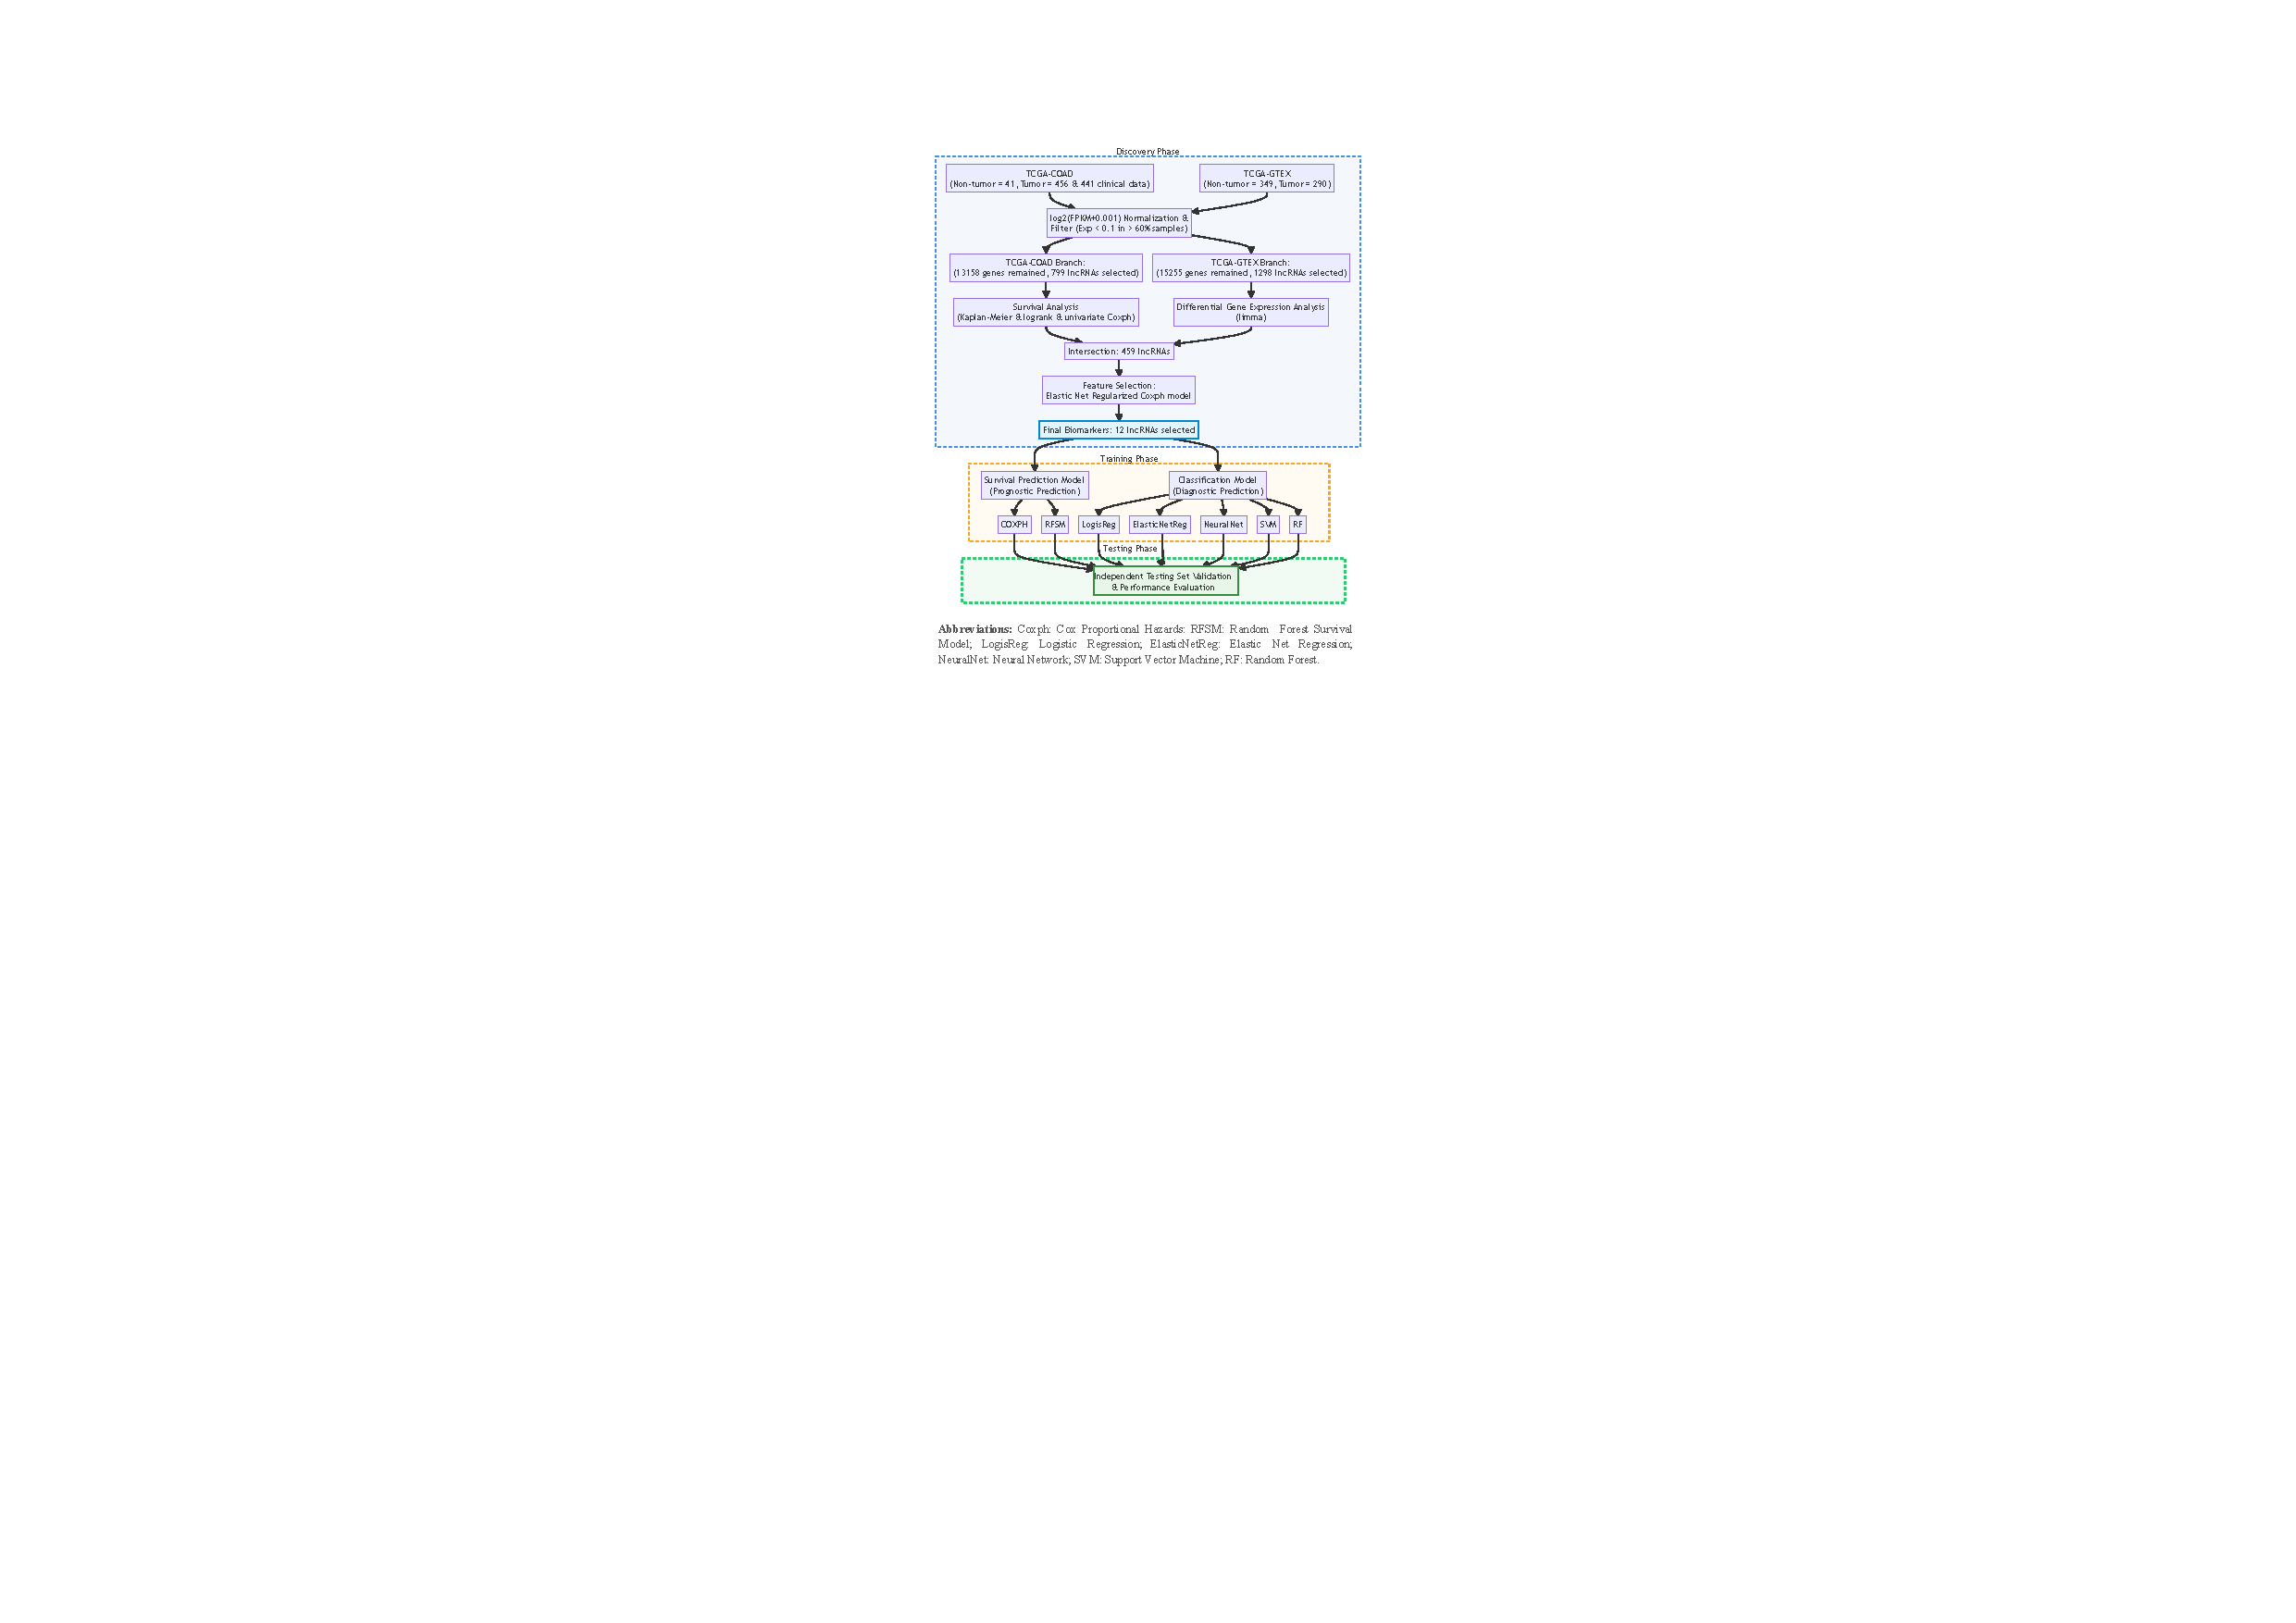
\includegraphics[width=0.92\textwidth, keepaspectratio]{Figure-1}
\caption{Study flowchart. The TOIL-recomputed TCGA--GTEx expression data (log$_2$(FPKM+0.001) normalized) was used for differential expression analysis and classification model training (639 samples). The original TCGA-COAD HTSeq-FPKM data was used for survival analysis and prognostic model construction (428 patients with complete clinical annotation). The pipeline integrates limma-based differential expression, elastic-net regularized Cox regression for feature selection, multivariate Cox and random survival forest modeling for prognosis, and five machine learning classifiers for diagnosis.}
\label{Fig1}
\end{figure}

\begin{figure}[!htp]
\centering
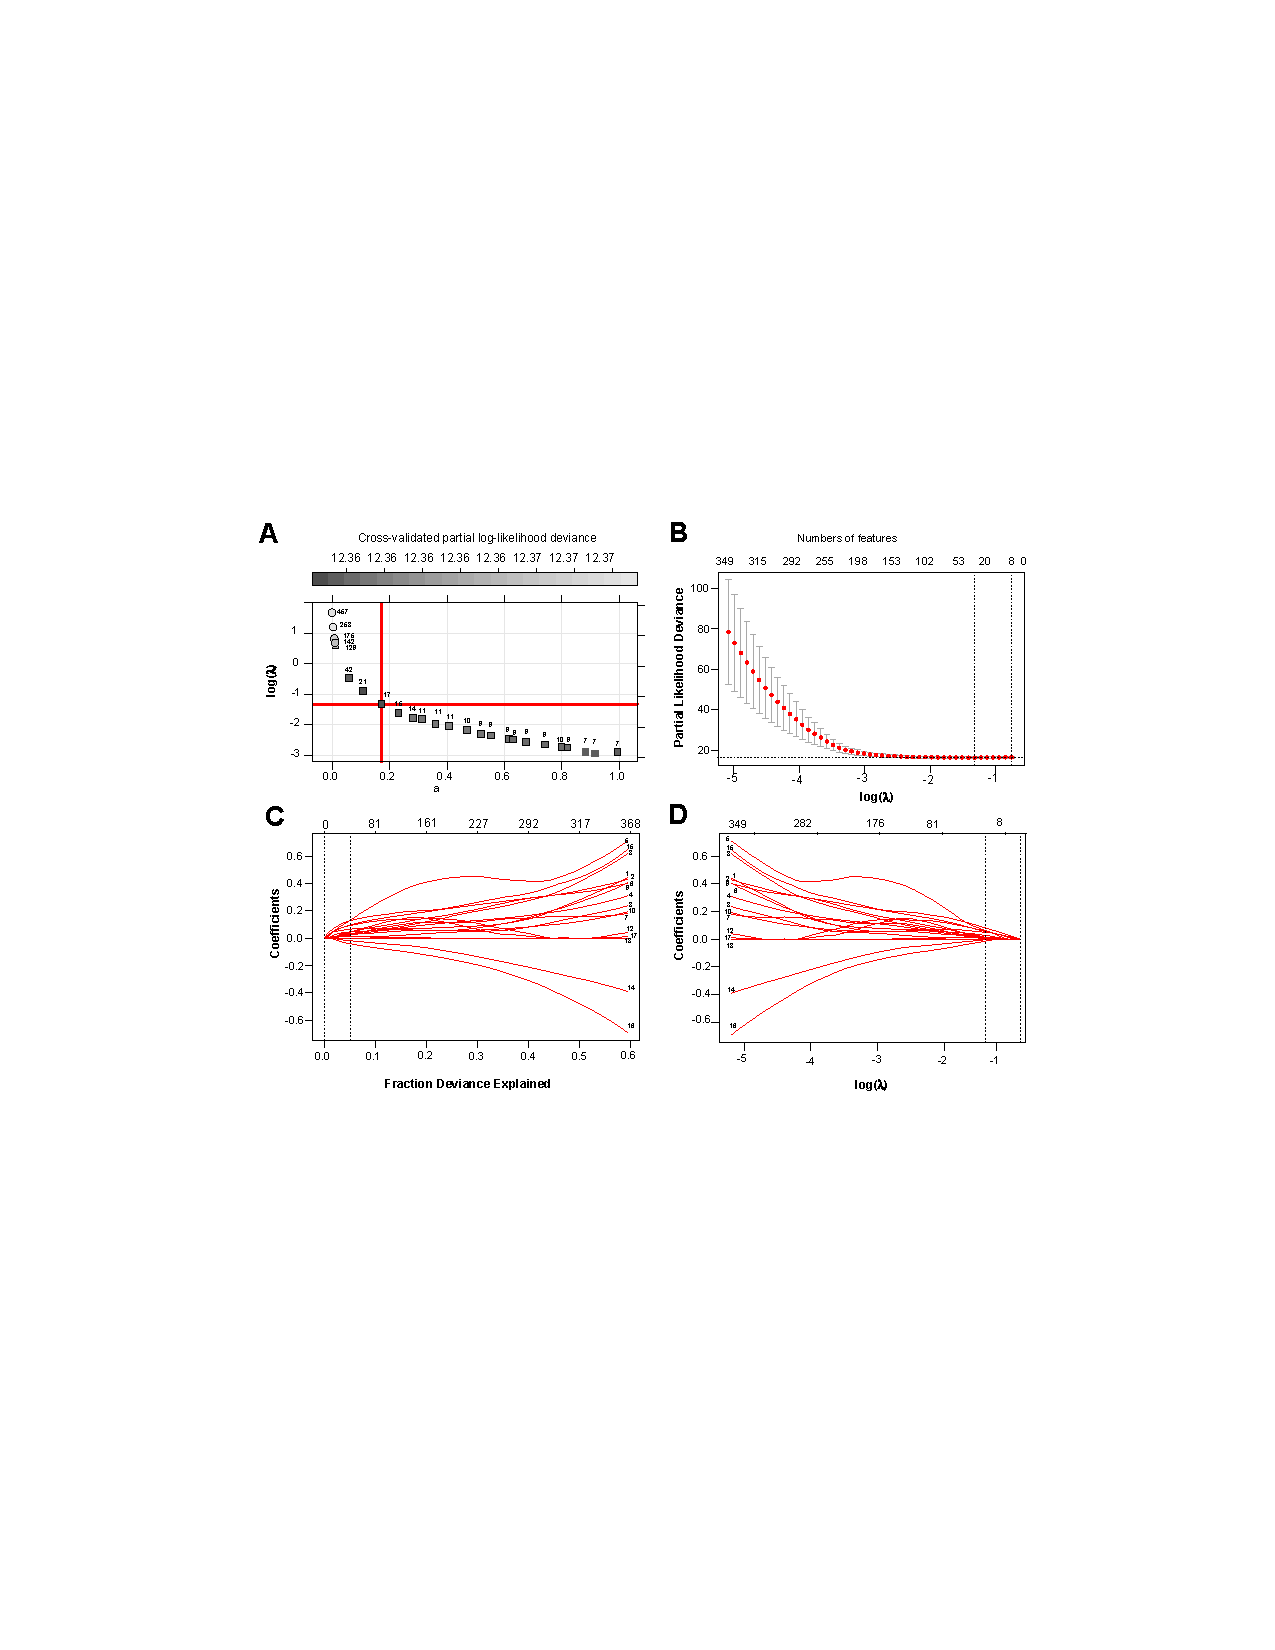
\includegraphics[width=1\textwidth, keepaspectratio]{Figure-2}
\caption{Elastic-net regularized Cox regression for lncRNA feature selection. (a) Three-dimensional surface of cross-validated partial log-likelihood deviance as a function of $\alpha$ and $\lambda$, with the optimal parameters marked ($\alpha = 0.200$, $\lambda = 0.230$, minimum deviance = 2.588). (b) Cross-validated partial likelihood deviance curve for the optimal $\alpha$ value; the left dotted line indicates $\lambda_{\min}$ and the right line indicates $\lambda_{\mathrm{1se}}$. (c) Coefficient shrinkage paths as a function of $\log(\lambda)$; red paths indicate the 17 lncRNAs with non-zero coefficients at $\lambda_{\min}$. (d) Coefficient shrinkage as a function of fraction deviance explained; the right dashed line indicates the null model.}
\label{Fig2}
\end{figure}

\subsection*{Prognostic model construction and evaluation}

The 428-patient cohort was randomly partitioned into training (70\%, n = 300) and testing (30\%, n = 128) sets, stratified by vital status. Baseline characteristics were well balanced between groups (Table~S1). We applied stepwise multivariate Cox regression (bidirectional selection, AIC minimization) to the 17 candidate lncRNAs and pathological stage in the training set, yielding a final model of 11 features: 8 lncRNAs and stage (as a 4-level factor, reference = Stage I). The final model achieved an AIC of 615.76 and a C-index of 0.82 in the training set. Variables with statistically significant hazard ratios under the Wald test included Stage IV (HR = 9.65, 95\% CI: 2.20--42.36, $p = 0.003$), RP11-440D17.3 (HR = 1.18, 95\% CI: 1.05--1.33, $p = 0.005$), MIR210HG (HR = 1.52, 95\% CI: 1.18--1.96, $p = 0.001$), and EIF3J-AS1 (HR = 1.35, 95\% CI: 1.08--1.68, $p = 0.009$), as shown in the forest plot (Fig.~\ref{Fig3}).

A relative risk score (RRS) was calculated from the Cox model for each patient. The RRS successfully stratified patients into high- and low-risk groups with significantly distinct overall survival in both the training set (log-rank $p < 0.0001$) and the testing set (log-rank $p = 0.0028$), as illustrated by Kaplan--Meier curves (Fig.~\ref{Fig4}a,b). Death events were substantially enriched in the high-risk group (77.7\% vs. 22.3\% in the low-risk group; Table~S2).

Time-dependent receiver operating characteristic (ROC) analysis demonstrated that the RRS served as an excellent metric for risk prediction over time. The area under the curve (AUC) was 0.754 (1-year), 0.738 (3-year), and 0.731 (5-year) in the training set, and 0.712 (1-year), 0.698 (3-year), and 0.685 (5-year) in the testing set (Fig.~\ref{Fig5}a--c). Longitudinal AUC analysis revealed that prediction performance gradually stabilized over time, with AUC values in both groups converging to approximately 0.725 at 8 years post-diagnosis (Fig.~\ref{Fig5}d).

\begin{figure}[!htp]
\centering
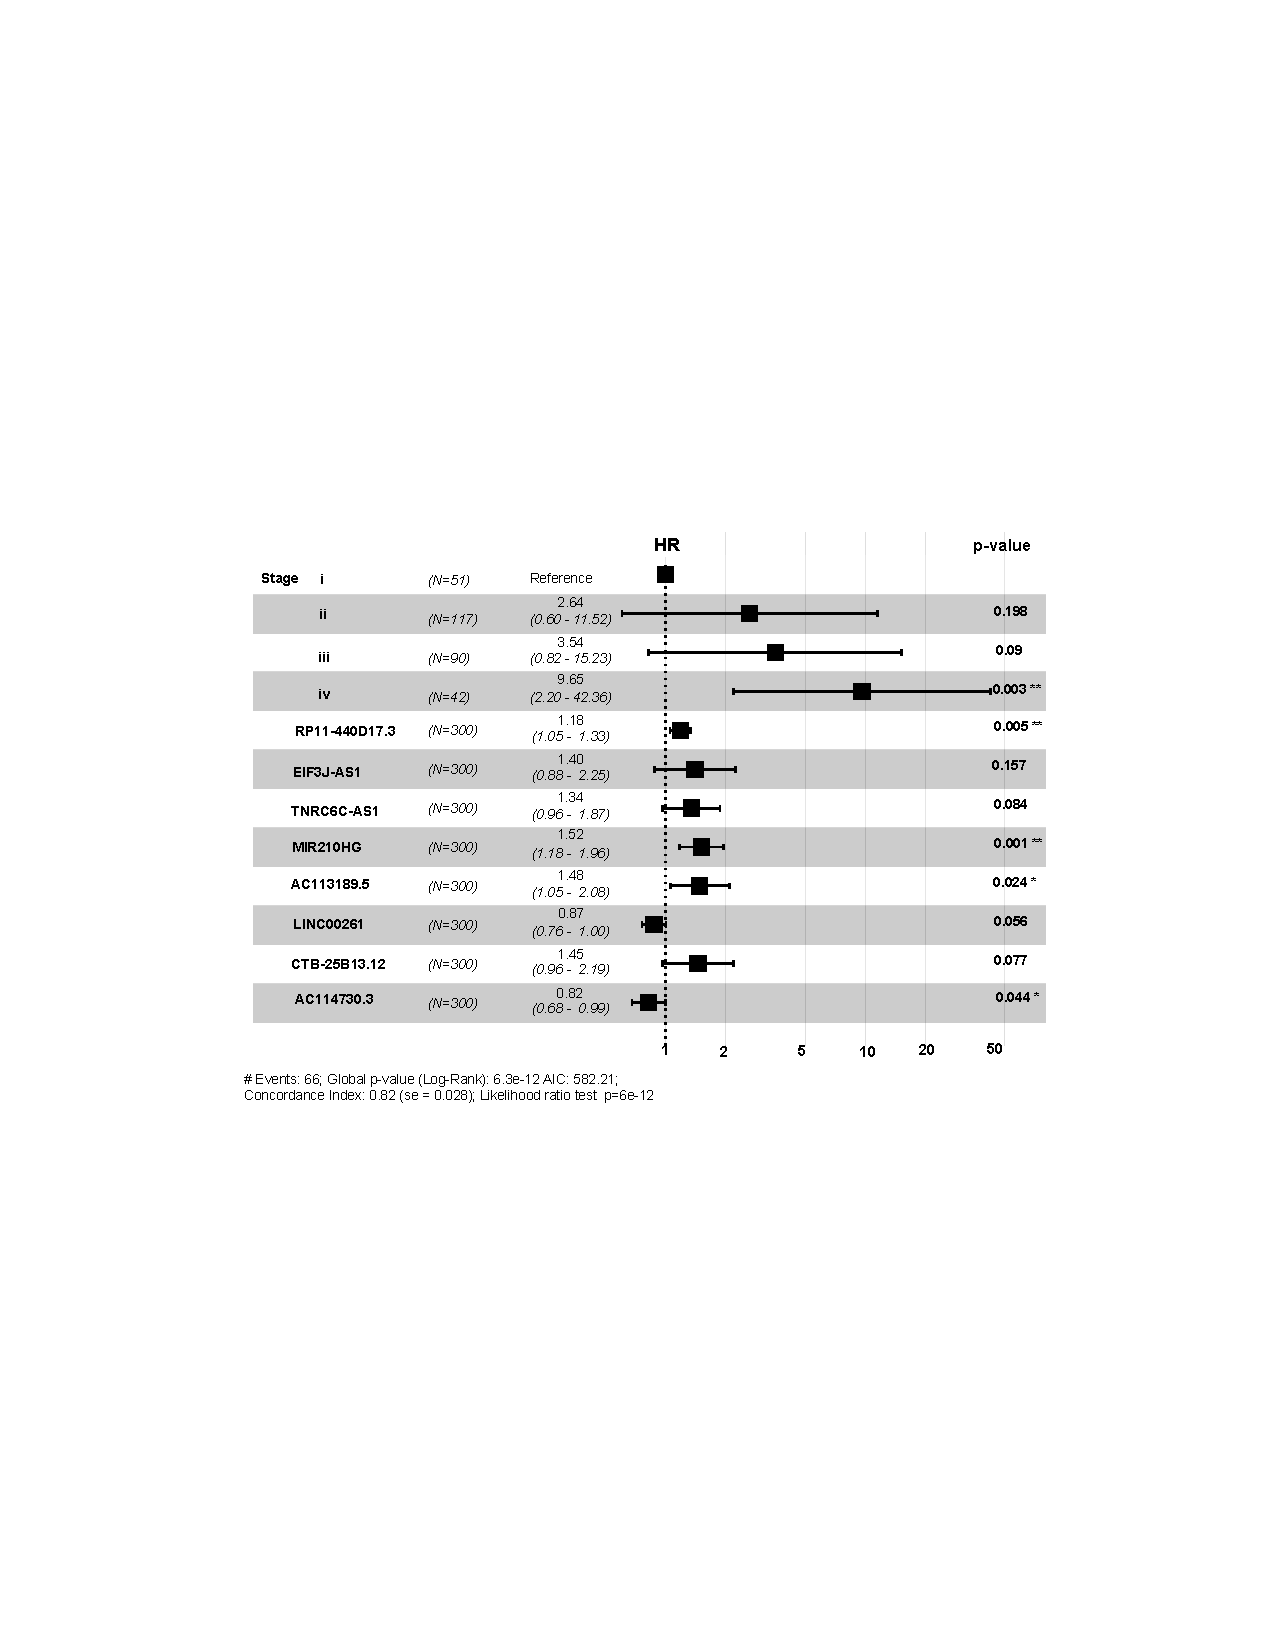
\includegraphics[width=1\textwidth]{Figure-3}
\caption{Forest plot of the multivariate Cox proportional hazards model. Hazard ratios (black squares) are shown with 95\% confidence intervals. Stage IV (HR = 9.65), RP11-440D17.3 (HR = 1.18), MIR210HG (HR = 1.52), and EIF3J-AS1 (HR = 1.35) were statistically significant predictors of overall survival under the Wald test. Stage I served as the reference category. The model C-index was 0.82 in the training cohort.}
\label{Fig3}
\end{figure}

\begin{figure}[!htp]
\centering
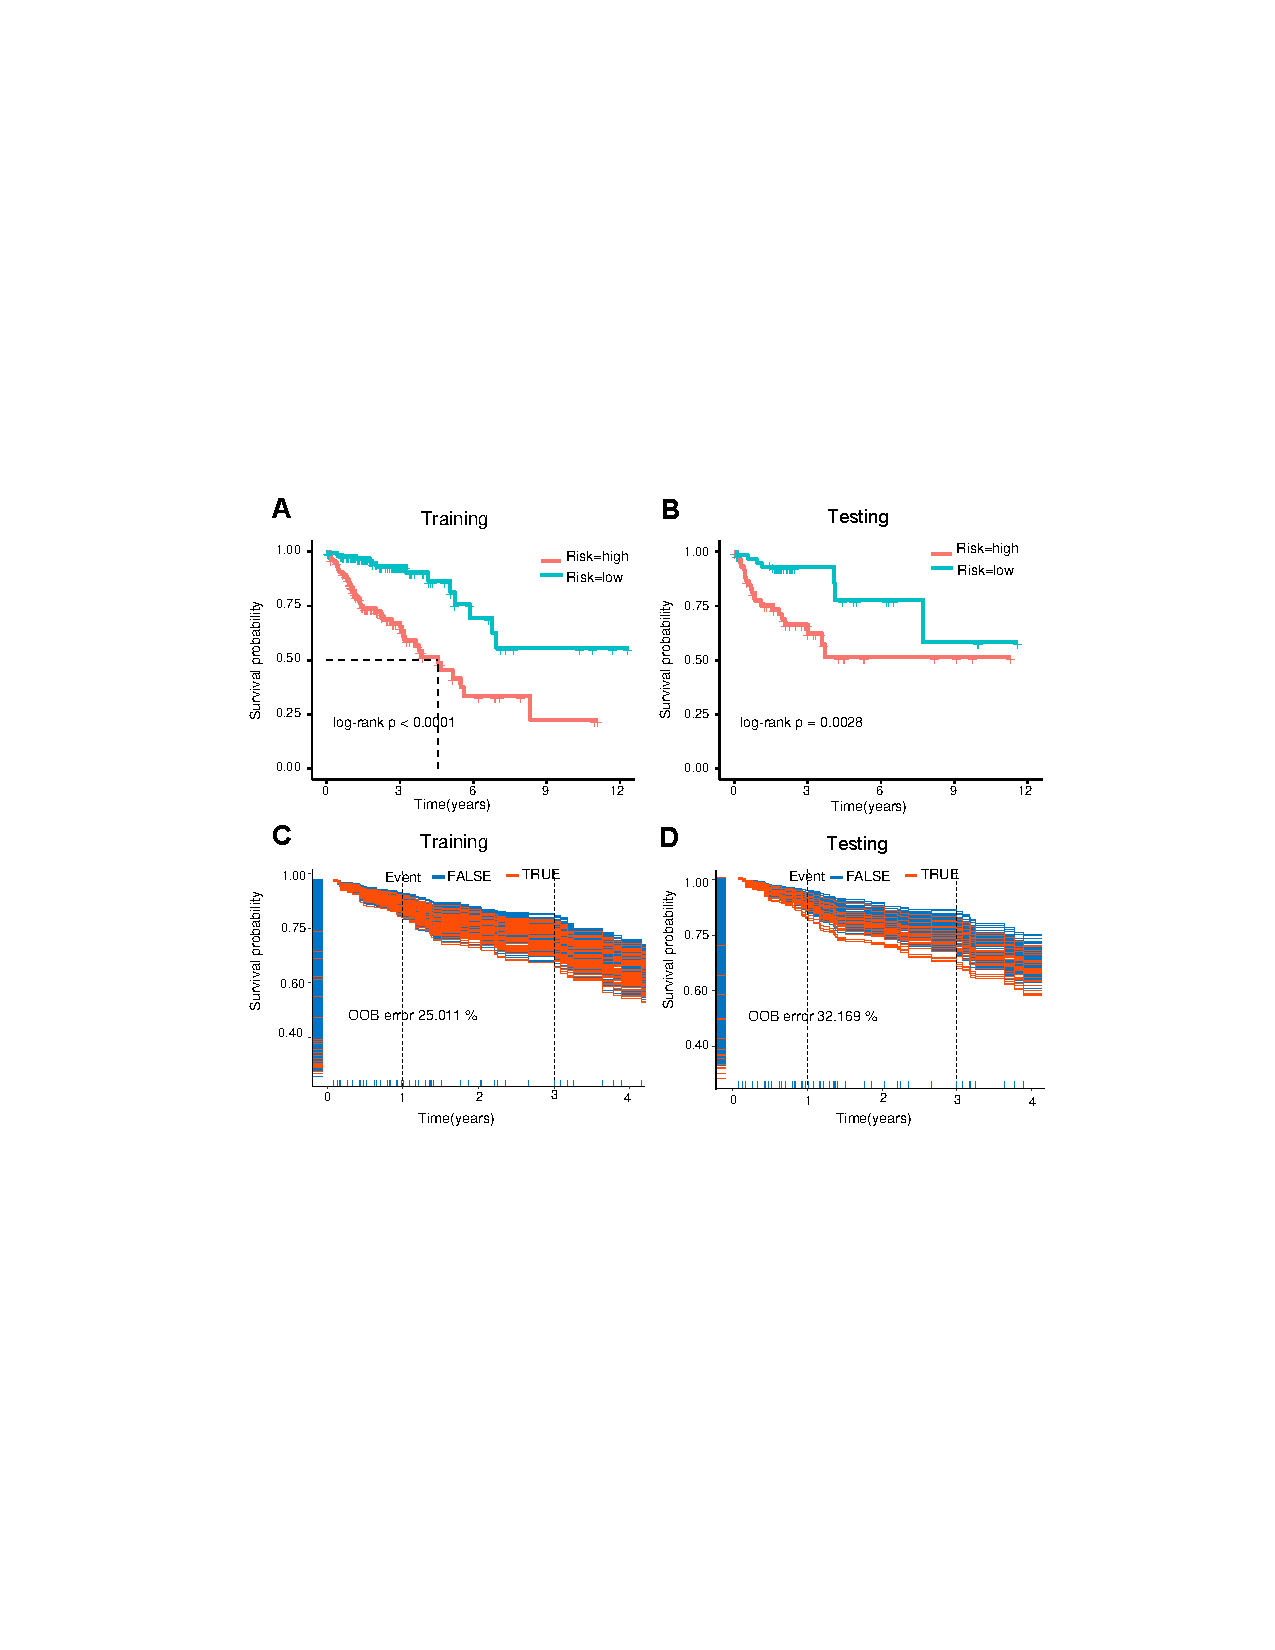
\includegraphics[width=1\textwidth]{Figure-4}
\caption{Risk stratification and survival prediction. (a,b) Kaplan--Meier curves for patients stratified into high- and low-risk groups by the Cox risk score in the training (a) and testing (b) sets. $P$-values are from the log-rank test. (c,d) Random forest predicted survival in training (c) and testing (d) sets. Blue lines correspond to censored observations; red lines correspond to patients experiencing the event (death). Dashed vertical lines indicate 1- and 3-year survival estimates. OOB error rates are 25.0\% (training) and 32.2\% (testing).}
\label{Fig4}
\end{figure}

\begin{figure}[!htp]
\centering
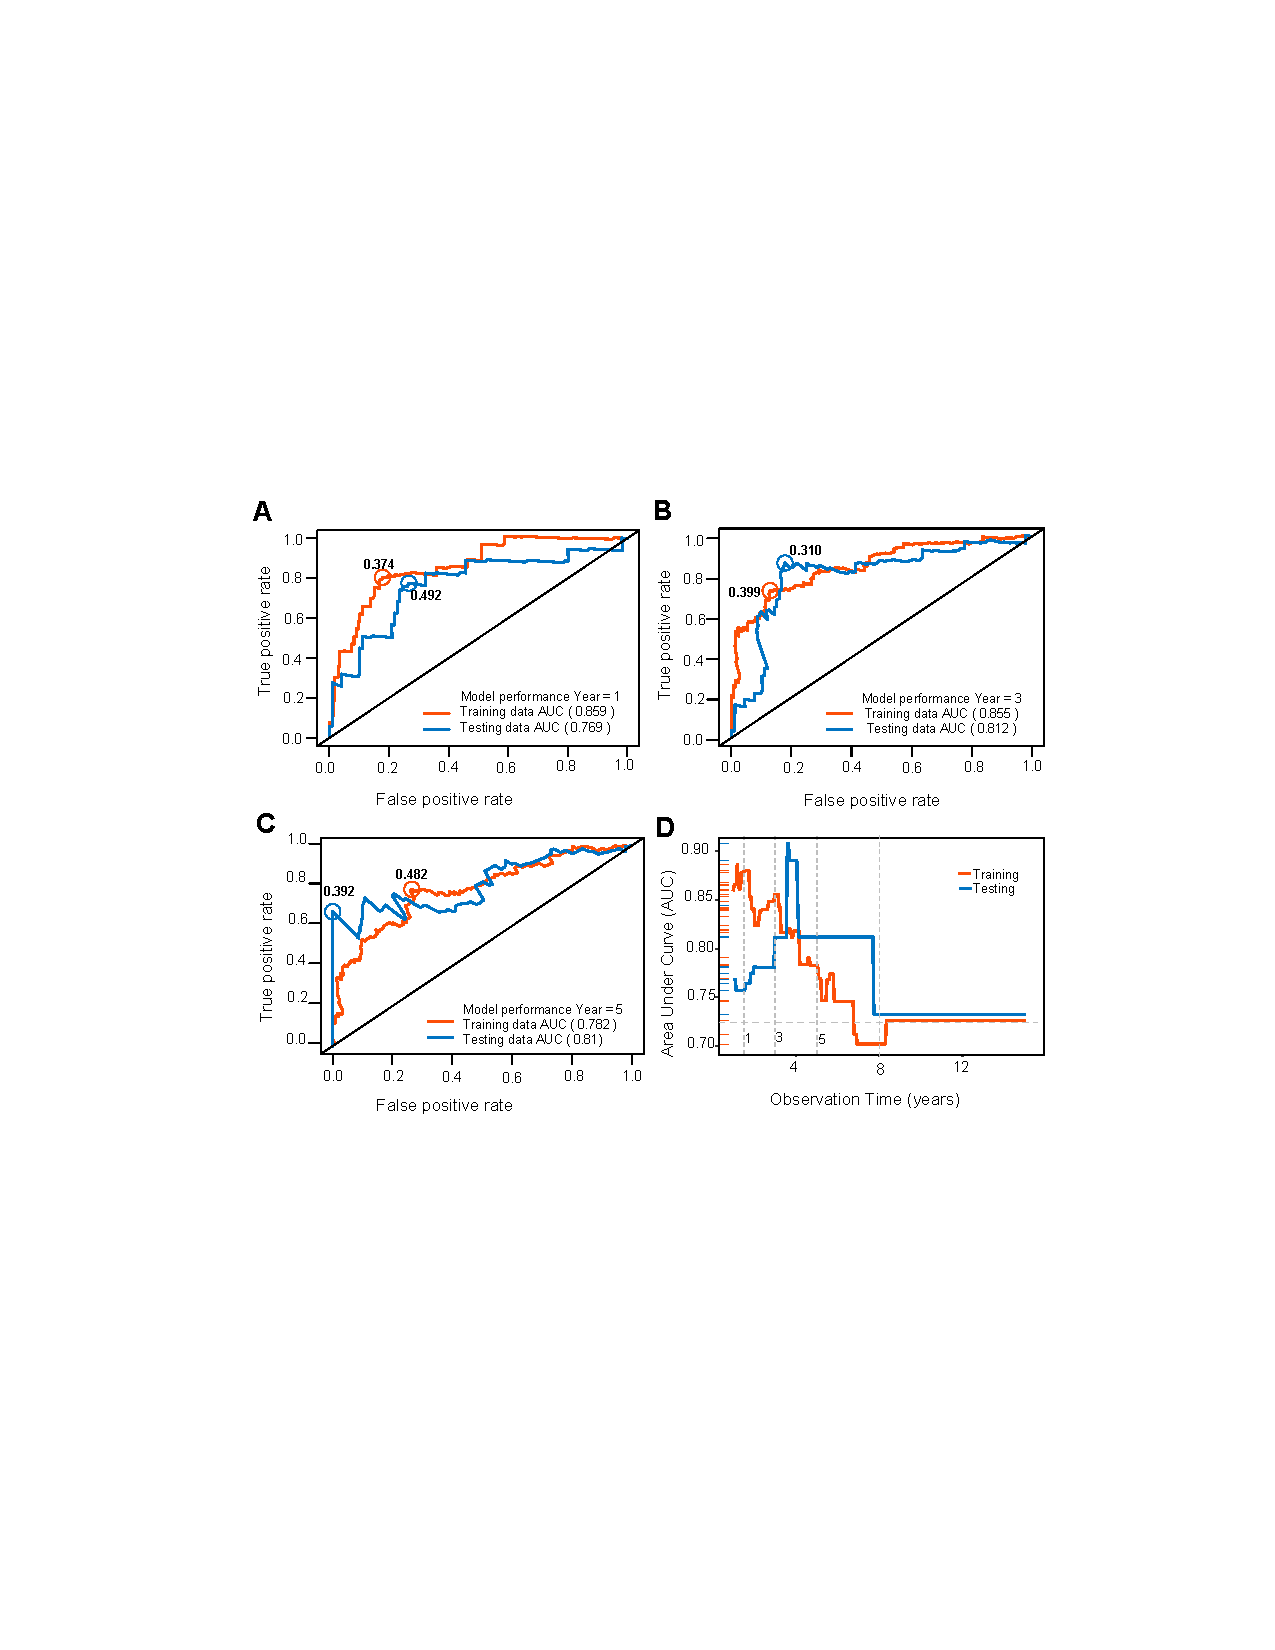
\includegraphics[width=1\textwidth]{Figure-5}
\caption{Time-dependent ROC analysis of the Cox risk prediction model. (a--c) ROC curves at 1, 3, and 5 years for training (blue) and testing (red) sets, with optimal thresholds marked. (d) Longitudinal AUC over 15 years of observation. AUC values in both groups converge to approximately 0.725 at 8 years, demonstrating stable long-term prognostic performance.}
\label{Fig5}
\end{figure}

\subsection*{Random forest survival analysis}

To provide a complementary non-parametric approach, we constructed a random survival forest (RSF) model using the same 8 lncRNA features and stage. Hyperparameter tuning identified optimal parameters of mtry = 1 and nodesize = 2, with 500 trees grown under a log-rank splitting rule. The RSF achieved an out-of-bag (OOB) error rate of 25.0\% in the training set, but this increased to 32.2\% in the testing set (Fig.~\ref{Fig4}c,d), indicating moderate overfitting consistent with the relatively small feature set limiting ensemble diversity.

Variable importance analysis by permutation identified stage as the dominant predictor (relative importance = 1.000), followed by LINC00261 (0.441), MIR210HG (0.370), and TNRC6C-AS1 (0.354) (Fig.~S2). Prediction error was evaluated using the time-dependent Brier score and concordance index (C-index) with 100 bootstrap cross-validation iterations. The Cox model incorporating lncRNA expression consistently outperformed both the stage-only Cox model and the random forest across the full observation period (Fig.~\ref{Fig6}). This indicates that (i) adding lncRNA expression information improves prognostic accuracy beyond stage alone, and (ii) the proportional hazards assumption is reasonable for this lncRNA signature, giving Cox regression an advantage over the more flexible but data-hungry random forest approach.

\begin{figure}[!htp]
\centering
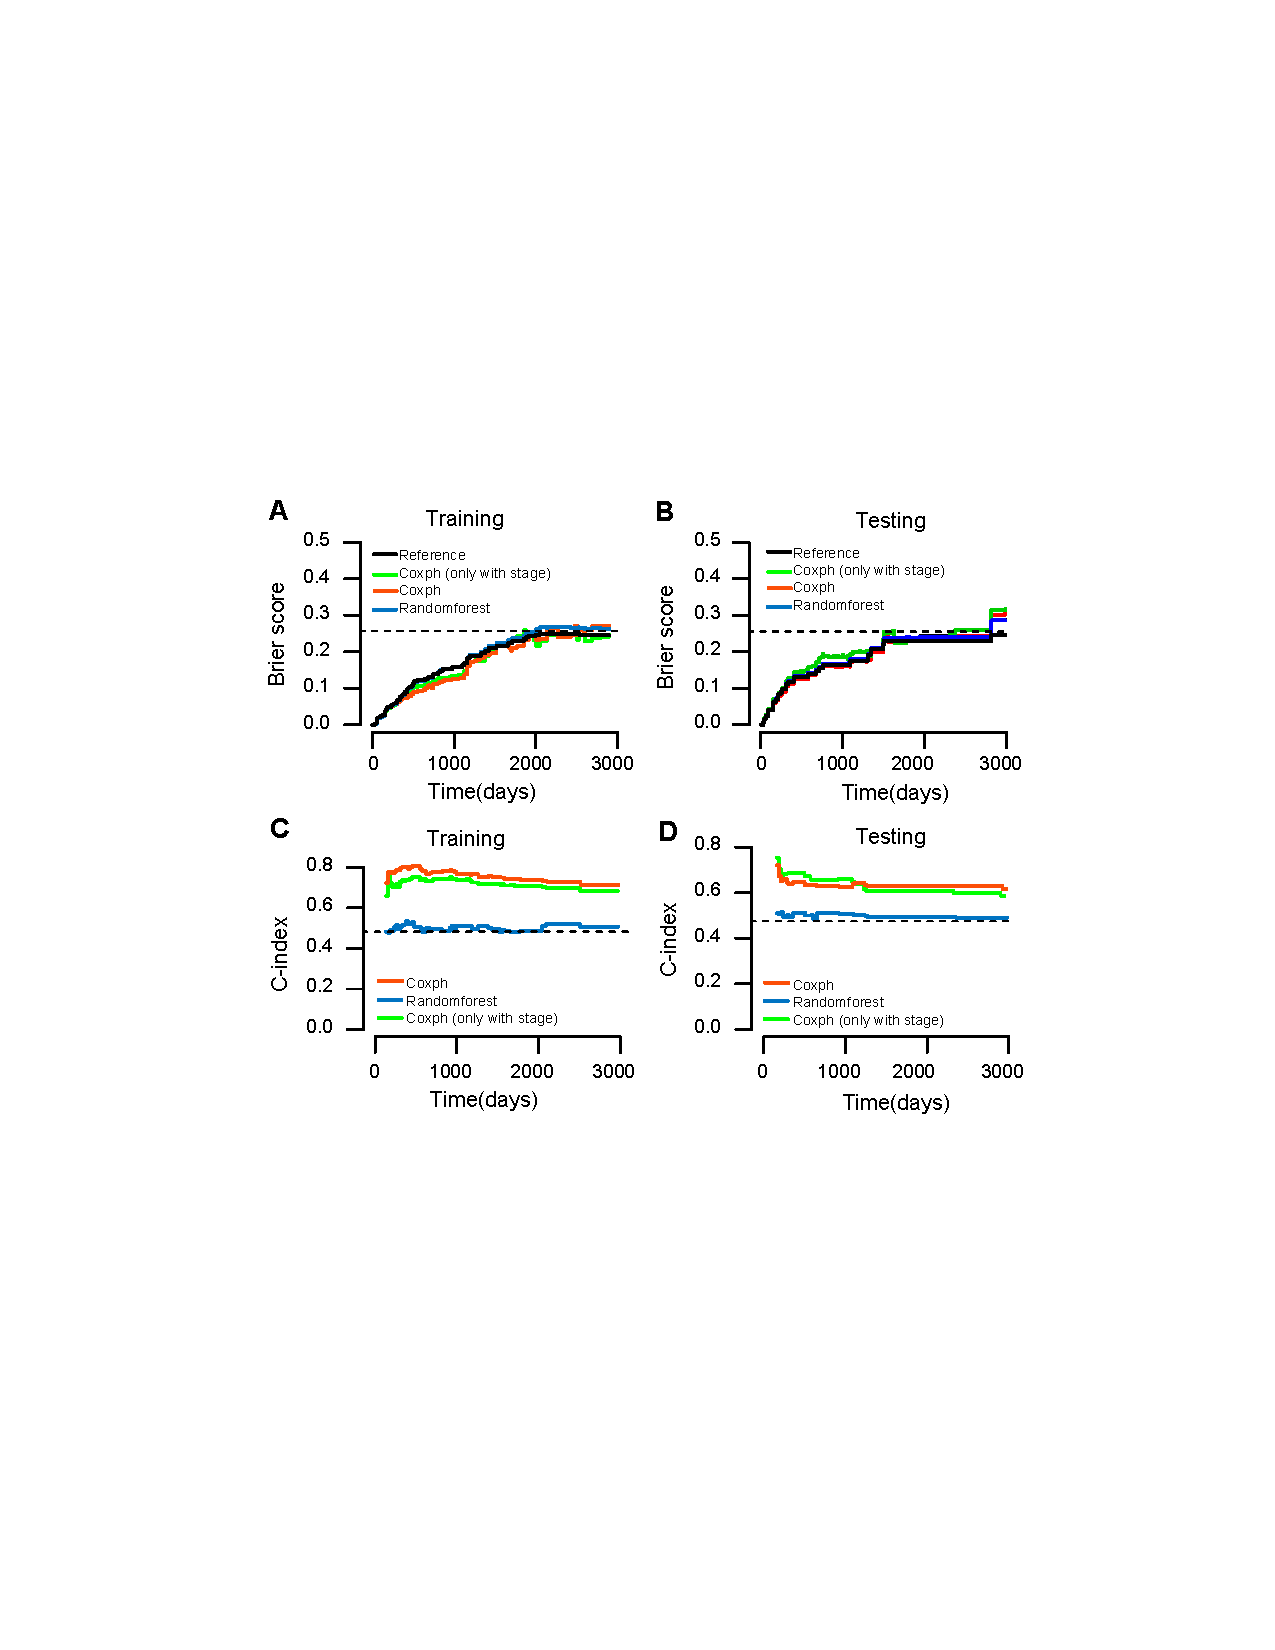
\includegraphics[width=1\textwidth]{Figure-6}
\caption{Model performance comparison for time-dependent risk prediction. (a,b) Brier score (prediction error) over time for the Cox model with stage only, Cox model with stage and lncRNAs, and random forest, in training (a) and testing (b) sets. Lower Brier scores indicate better calibration. (c,d) Concordance index (C-index) over time in training (c) and testing (d) sets. Higher C-index indicates better discrimination. Adding lncRNA expression improved both calibration and discrimination beyond stage alone, and Cox regression outperformed random forest across all time points.}
\label{Fig6}
\end{figure}

\subsection*{Classification models for diagnostic prediction}

The 8 lncRNAs selected by the prognostic pipeline were further evaluated for their diagnostic utility in distinguishing tumor from non-tumor samples. Using the TCGA--GTEx expression data (639 samples: 349 non-tumor, 290 tumor), we trained five classification models with 10-fold cross-validation repeated 5 times: support vector machine with radial basis kernel (SVM), random forest (RF), neural network (NNET), elastic-net regularized logistic regression, and logistic regression with stepwise AIC selection. Features were Box-Cox transformed prior to modeling.

The performance of all classifiers is summarized in Table~\ref{Tab2} and Fig.~\ref{Fig7}. SVM, RF, and NNET all achieved excellent discriminative performance, with testing-set accuracies of 92.1\%, 91.1\%, and 92.1\%, respectively, and AUC values of 0.969, 0.974, and 0.973. These three strong classifiers exhibited high precision (0.90--0.93) and recall (0.89--0.93), with Kappa statistics exceeding 0.82, indicating excellent agreement beyond chance. In contrast, linear models performed substantially worse: logistic regression achieved 64.9\% testing accuracy (AUC = 0.761) and elastic-net logistic regression 64.4\% (AUC = 0.765), suggesting that the decision boundaries between tumor and normal lncRNA expression patterns are fundamentally non-linear.

Lift curve analysis confirmed that SVM, RF, and NNET captured the majority of tumor-positive samples within the top percentile bins, substantially outperforming random selection, while logistic and elastic-net models showed more modest improvements over baseline (Fig.~\ref{Fig7}c,d).

\begin{figure}[!htp]
\centering
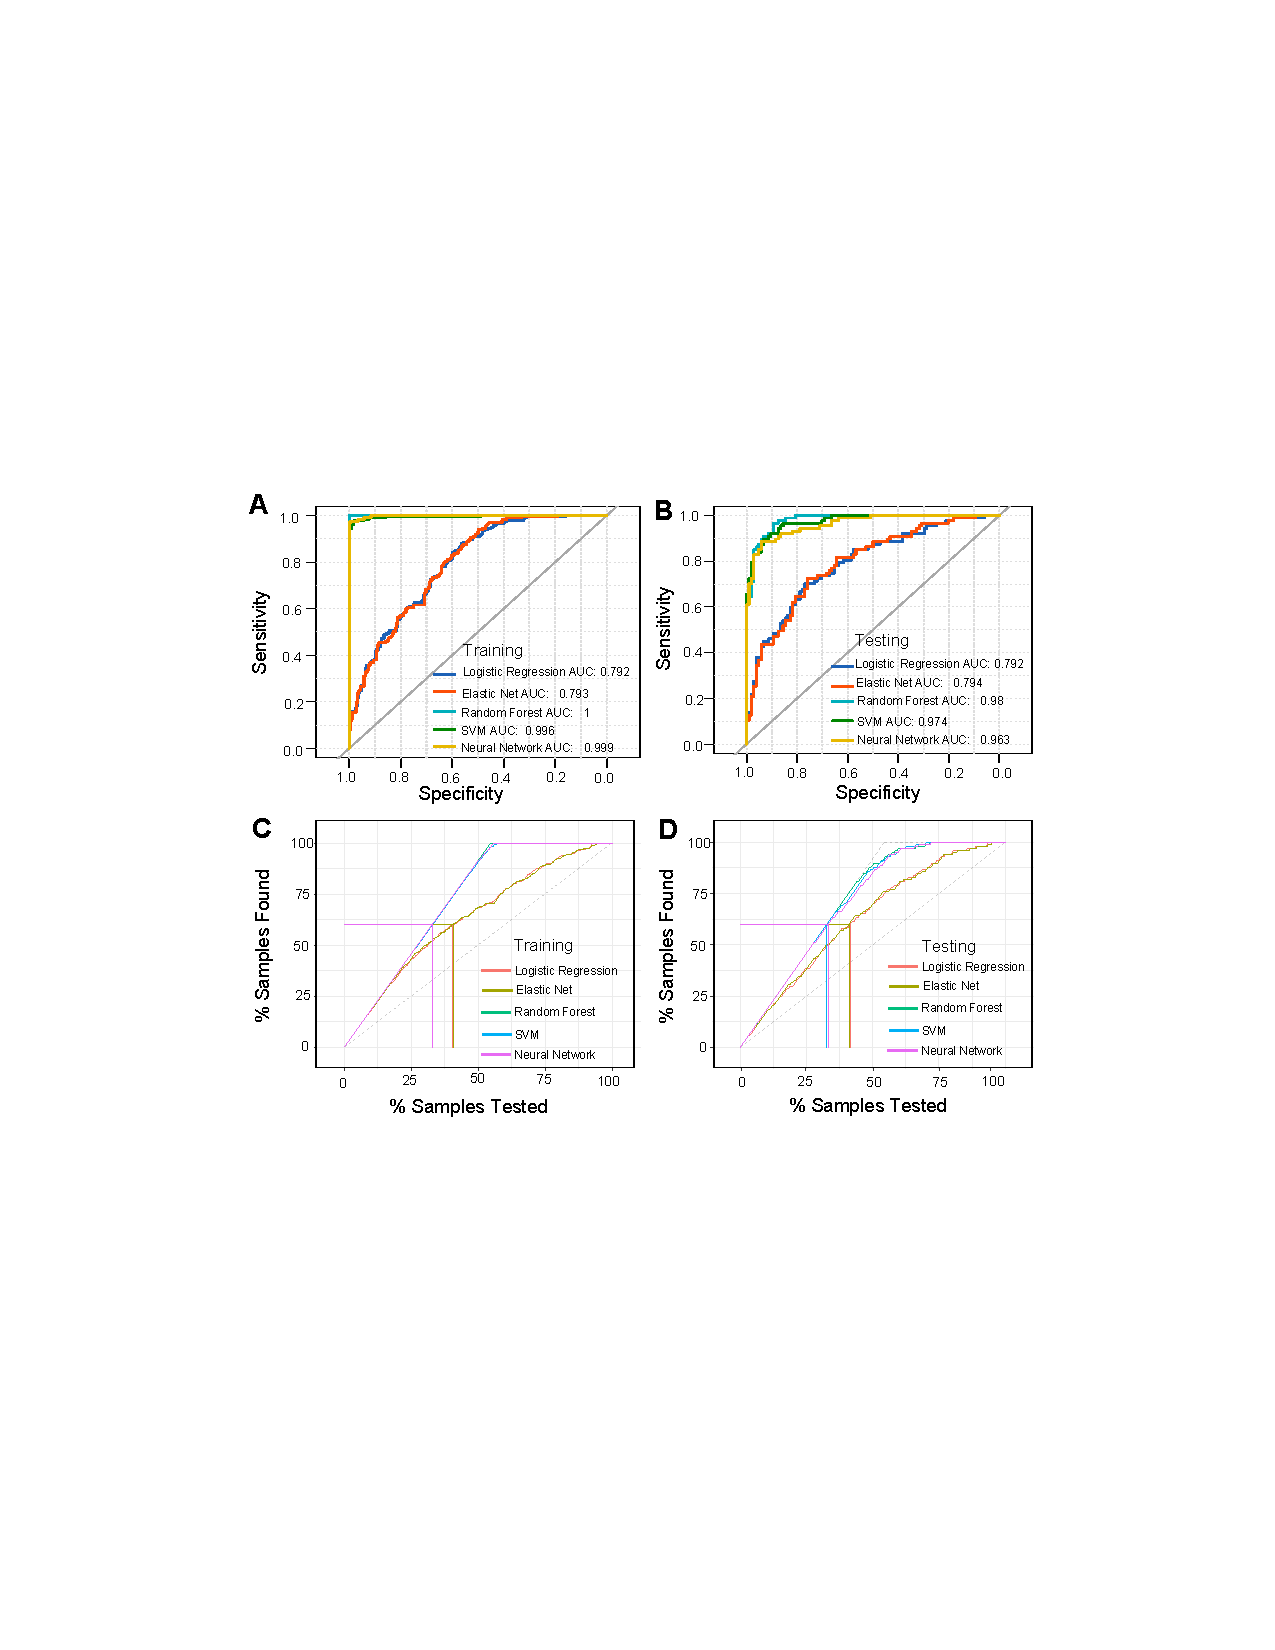
\includegraphics[width=1\textwidth]{Figure-7}
\caption{ROC and lift curves for classification models. (a,b) ROC curves for all five classifiers in training (a) and testing (b) sets. SVM, random forest, and neural network achieved AUC values approaching 1.0, while logistic regression and elastic-net models exhibited substantially lower discriminative performance. (c,d) Cumulative lift curves in training (c) and testing (d) sets. Strong classifiers showed enhanced response rates compared to the random baseline (dashed diagonal), successfully capturing most events within a small fraction of the ranked samples.}
\label{Fig7}
\end{figure}

\begin{table}[htp]
  \setlength\tabcolsep{1.8pt}
  \centering
  \caption{Performance of classification models on training and testing data.}
    \begin{tabular}{llcccccc}
        \toprule[2pt]
   \rowcolor{Blue}\textbf{Classifier} & \textbf{Set} & \textbf{Accuracy} & \textbf{AUC} & \textbf{Precision} & \textbf{Recall} & \textbf{F1} & \textbf{Kappa} \\
         \midrule[1pt]
    Logistic Reg. & Train & 0.763 & 0.839 & 0.728 & 0.764 & 0.745 & 0.525 \\
          & Test & 0.649 & 0.761 & 0.614 & 0.621 & 0.617 & 0.293 \\
    Elastic Net & Train & 0.757 & 0.841 & 0.726 & 0.744 & 0.735 & 0.510 \\
          & Test & 0.644 & 0.765 & 0.612 & 0.598 & 0.605 & 0.281 \\
    \specialrule{0em}{.3em}{.3em}
   \rowcolor{LightBlue}\textbf{SVM} & Train & 0.971 & 0.997 & 0.952 & 0.985 & 0.969 & 0.942 \\
       \rowcolor{LightBlue}   & Test & \textbf{0.921} & 0.969 & 0.900 & 0.931 & 0.915 & 0.842 \\
    \specialrule{0em}{.3em}{.3em}
    \textbf{Random Forest}& Train & 1.000 & 1.000 & 1.000 & 1.000 & 1.000 & 1.000 \\
         & Test & 0.911 & \textbf{0.974} & 0.917 & 0.885 & 0.901 & 0.820 \\
    \specialrule{0em}{.3em}{.3em}
   \rowcolor{LightBlue}\textbf{Neural Net}& Train & 0.969 & 0.995 & 0.975 & 0.956 & 0.965 & 0.937 \\
       \rowcolor{LightBlue}   & Test & \textbf{0.921} & 0.973 & \textbf{0.929} & \textbf{0.897} & \textbf{0.912} & 0.841 \\
          \bottomrule[1.5pt]
    \end{tabular}
  \label{Tab2}
\end{table}

\subsection*{Biological relevance of identified lncRNAs}

To assess whether the lncRNAs selected by our pipeline have established biological functions in cancer, we conducted a comprehensive literature survey. Notably, the top-ranked lncRNA in our univariate Cox analysis, MIR210HG (HR = 1.40, 95\% CI: 1.17--1.69, $p = 0.0003$), has been extensively characterized in CRC. MIR210HG is consistently upregulated in CRC tissues, serum, and cell lines, and functions as an oncogenic transcript through at least two distinct mechanisms: acting as a competing endogenous RNA (ceRNA) sponge for miR-1226-3p to promote proliferation and inhibit apoptosis, and binding directly to PCBP1 (the primary cytoplasmic iron chaperone) to suppress ferroptosis via upregulation of GPX4\cite{RN20,RN21}. Its transcription is activated by the CREB3 transcription factor. Clinically, high MIR210HG expression is independently associated with poor overall survival (multivariate HR = 3.93, $p = 0.014$) and elevated serum MIR210HG achieves a diagnostic AUC of 0.870.

Several other lncRNAs in our signature have established cancer relevance. EIF3J-AS1 (also known as EIF3J-DT; HR = 1.70, $p = 0.0036$) was recently shown to induce chemoresistance in gastric cancer by activating autophagy through dual regulation of ATG14 --- directly stabilizing ATG14 mRNA and sponging miR-188-3p to block miRNA-mediated degradation\cite{RN22}. It is also upregulated in hepatocellular carcinoma and esophageal cancer. LINC00261 (HR = 0.90, $p = 0.022$), one of the two protective lncRNAs in our signature, is a well-documented tumor suppressor: it physically binds the Slug (SNAI2) protein and promotes its degradation by enhancing the GSK3$\beta$--Slug interaction, thereby suppressing epithelial-mesenchymal transition and metastasis\cite{RN23}. CD27-AS1 (HR = 1.80, $p = 0.0010$), the lncRNA with the highest hazard ratio among our top candidates, is an immune-related antisense transcript to the TNF receptor family member CD27. It has been shown to drive AML progression through the miR-224-5p/PBX3/MAPK signaling axis and to promote melanoma proliferation via STAT3 interaction\cite{RN24}. PCAT6 (HR = 1.40, $p = 0.0025$) is a well-established pan-cancer oncogenic lncRNA that functions primarily as a ceRNA, sponging multiple tumor-suppressive miRNAs to derepress oncogenic targets including HMGA2 and EZH2\cite{RN25}. In CRC specifically, PCAT6 promotes epithelial-mesenchymal transition, stemness, and 5-fluorouracil chemoresistance.

Importantly, several lncRNAs that ranked highly in our analysis have no prior functional characterization in any cancer type. CTB-25B13.12 (HR = 1.70, $p = 0.0004$), AP006621.5 (HR = 1.60, $p = 0.0003$), RP11-549B18.1 (HR = 0.71, $p = 0.0052$), and RP11-440D17.3 (HR = 1.10, $p = 0.064$, selected in the final Cox model) represent genuinely novel candidates that merit experimental validation. Their strong statistical association with CRC survival in our analysis, combined with their selection by rigorous machine learning procedures, positions them as high-priority targets for functional investigation.

\section*{Discussion}

In this study, we developed and applied a comprehensive, reproducible machine learning pipeline to discover lncRNA signatures with dual diagnostic and prognostic value in colorectal cancer. Our analysis integrated differential expression profiling of 639 samples, elastic-net regularized survival modeling of 428 patients, and five classification algorithms, yielding an 8-lncRNA panel that demonstrated robust performance across both diagnostic and prognostic tasks.

Several aspects of our analytical approach merit discussion. First, the use of the TOIL-recomputed TCGA--GTEx dataset for differential expression analysis provided substantial statistical power with 349 non-tumor and 290 tumor samples, compared to the 41 adjacent normal samples in the original TCGA-COAD dataset. This harmonized resource, combined with GENCODE v22/v23 lncRNA annotations, enabled confident identification of differentially expressed lncRNAs. Second, our elastic-net grid search identified an optimal $\alpha$ of 0.200, substantially closer to ridge ($\alpha = 0$) than lasso ($\alpha = 1$) regularization. This indicates that lncRNA expression features in CRC are highly inter-correlated, consistent with the biology of co-expressed lncRNA networks sharing common transcriptional regulatory mechanisms. The ridge-dominant penalty appropriately retains correlated features rather than arbitrarily selecting one representative from each correlated group. Third, the subsequent stepwise Cox refinement reduced the 17 elastic-net-selected lncRNAs to 8 in the final model (plus stage), balancing parsimony with predictive performance.

From a biological perspective, the concordance between our computational findings and existing literature is noteworthy. MIR210HG, our most statistically significant lncRNA, has been functionally validated in CRC through two independent mechanisms --- ferroptosis inhibition via PCBP1 binding and ceRNA activity via miR-1226-3p sponging --- with clinical evidence supporting its diagnostic and prognostic utility. Similarly, the tumor-suppressive function of LINC00261 through Slug degradation, the autophagy-mediated chemoresistance mechanism of EIF3J-AS1, and the immune-modulatory role of CD27-AS1 all align with the direction and magnitude of hazard ratios observed in our analysis. This concordance between computational prediction and experimental validation strengthens confidence in our pipeline's ability to identify biologically meaningful biomarkers.

Equally important are our novel findings. CTB-25B13.12 (HR = 1.70, the third most significant lncRNA in our analysis), AP006621.5 (HR = 1.60), and RP11-549B18.1 (HR = 0.71, the strongest protective signal) have no published functional studies in any cancer type. These lncRNAs were selected through rigorous, multi-stage statistical filtering (differential expression $\rightarrow$ univariate Cox $\rightarrow$ elastic-net regularization $\rightarrow$ stepwise multivariate Cox) and represent genuine discovery candidates. Their strong and consistent association with CRC survival, reproducible across our fully documented pipeline, warrants prioritized experimental investigation.

The classification results revealed a clear dichotomy: strong non-linear classifiers (SVM, RF, NNET) achieved testing accuracies above 91\%, while linear models (logistic regression, elastic-net logistic regression) stagnated at approximately 65\%. This performance gap strongly suggests that the decision boundaries separating tumor from normal lncRNA expression states are fundamentally non-linear, likely reflecting the combinatorial and epistatic nature of lncRNA regulatory networks. The excellent generalization of SVM and NNET from training to testing data (accuracy loss $<$ 6\%) indicates that overfitting was well controlled by the rigorous cross-validation scheme, despite the modest sample size relative to feature dimensionality.

Several limitations should be acknowledged. First, our analysis was performed on a single retrospective cohort (TCGA-COAD) and lacks external validation in independent datasets. While TCGA represents the largest publicly available CRC dataset with comprehensive lncRNA expression and clinical annotation, additional validation in cohorts such as GEO datasets or prospective clinical samples is necessary before clinical translation. Second, missing clinical data --- particularly for perineural invasion (59.8\% missing) and preoperative CEA (36.4\% missing) --- limited our ability to comprehensively adjust for all potential confounders in the survival analysis. Third, as an observational study using archival data, our findings demonstrate association rather than causation; functional experiments are required to establish mechanistic roles for the novel lncRNAs identified. Fourth, our random forest model exhibited moderate overfitting (OOB error gap of 7.2\% between training and testing), likely attributable to the small feature set (8 lncRNAs plus stage) limiting the diversity that ensemble methods depend on. Finally, technical factors such as differences in RNA-sequencing protocols between TCGA and GTEx, while mitigated by TOIL harmonization, may still influence cross-platform comparisons.

Future work should prioritize: (i) external validation of our lncRNA signature in independent CRC cohorts; (ii) functional characterization of the novel lncRNAs CTB-25B13.12, AP006621.5, and RP11-549B18.1 through knockdown/overexpression experiments in CRC cell lines; (iii) construction of an integrated clinical nomogram incorporating lncRNA expression with routine pathological parameters; and (iv) extension of the pipeline to other gastrointestinal malignancies to assess the tissue-specificity versus generalizability of the identified signatures.

\section*{Methods}

\subsection*{Data acquisition and preprocessing}

Gene expression data and clinical annotations for colorectal adenocarcinoma (COAD) were obtained from The Cancer Genome Atlas (TCGA) via the Genomic Data Commons portal (https://portal.gdc.cancer.gov/). Two expression datasets were used: (i) HTSeq-FPKM data from TCGA-COAD (479 tumor and 41 non-tumor samples) for survival analysis, and (ii) TOIL-recomputed RSEM FPKM data integrating TCGA-COAD and GTEx colon samples (331 TCGA and 308 GTEx; 639 total) for differential expression and classification analyses. The TOIL data were already $\log_2(\text{FPKM} + 0.001)$ normalized. HTSeq-FPKM data were $\log_2(\text{FPKM} + 0.001)$ transformed prior to analysis. GENCODE v22 and v23 long non-coding RNA annotations were used to extract lncRNA expression profiles. Clinical data including survival time, vital status, pathological stage, and other covariates were obtained from TCGA clinical and follow-up files. Genes with expression values below 0.1 in more than 60\% of samples were excluded to reduce noise from lowly expressed transcripts.

\subsection*{Differential expression analysis}

Differential expression between tumor and non-tumor samples was performed using the \texttt{limma} package in R (v4.6.0). The linear model was fit with empirical Bayes moderation (trend = TRUE, robust = TRUE), and $p$-values were adjusted for multiple testing using the Benjamini--Hochberg procedure. lncRNAs with adjusted $p < 0.05$ were considered differentially expressed. Expression fold changes are reported as $\log_2(\text{Tumor}) - \log_2(\text{NonTumor})$.

\subsection*{Survival analysis and feature selection}

Overall survival was defined as the interval from initial diagnosis to death or last follow-up. Univariate Cox proportional hazards regression and Kaplan--Meier log-rank tests (median-split high/low expression groups) were performed for each lncRNA. LncRNAs with complete differential expression and survival association data (n = 459) were included in regularized survival modeling.

Elastic-net regularized Cox regression was performed using the \texttt{glmnet} package. The mixing parameter $\alpha$ was optimized by grid search over $\{0, 0.1, \ldots, 1.0\}$ with tenfold cross-validation, selecting the combination of $\alpha$ and $\lambda$ that minimized the cross-validated partial log-likelihood deviance. To accelerate computation, the $\alpha$ grid was parallelized using the \texttt{foreach} and \texttt{doParallel} packages.

The cohort was randomly partitioned into training (70\%) and testing (30\%) sets stratified by vital status. Stepwise multivariate Cox regression (bidirectional selection, AIC minimization) was applied in the training set to refine the lncRNA panel. A risk score was computed for each patient as the linear predictor from the final Cox model. Time-dependent ROC analysis was performed using the \texttt{survivalROC} package.

\subsection*{Random forest survival analysis}

Random survival forests were constructed using the \texttt{randomForestSRC} package. Hyperparameters (mtry, nodesize) were tuned via grid search minimizing OOB error. The final model used 500 trees with a log-rank splitting rule. Variable importance was assessed by permutation. Time-dependent Brier scores were computed using \texttt{riskRegression::Score} with 100 bootstrap cross-validation iterations, and C-indices were computed using \texttt{pec::cindex}.

\subsection*{Classification models}

Five classifiers were trained on the TCGA--GTEx expression data using the 8 lncRNAs from the prognostic pipeline: support vector machine with radial basis kernel (\texttt{kernlab}), random forest (\texttt{ranger}), neural network (\texttt{nnet}), elastic-net regularized logistic regression (\texttt{glmnet}), and logistic regression with stepwise AIC selection (\texttt{MASS}). Features were Box-Cox transformed using \texttt{caret::preProcess}. Model training used 10-fold cross-validation repeated 5 times, with hyperparameter tuning via grid search. Performance was assessed by accuracy, AUC, precision, recall, F1 score, and Cohen's Kappa.

\subsection*{Reproducibility}

The complete analysis pipeline is provided as a single, self-contained R script (\texttt{pipeline.R}) with a fixed random seed (set.seed(12345)). All figures and tables presented in this manuscript can be regenerated by executing \texttt{Rscript pipeline.R} from the project directory. The pipeline was developed and tested using R 4.6.0 on Windows 11. Key package versions are recorded in the pipeline output.

\subsection*{Data availability}

TCGA-COAD data are publicly available from the Genomic Data Commons (https://portal.gdc.cancer.gov/). GTEx data are available from the GTEx Portal (https://gtexportal.org/). TOIL-recomputed expression data are available from the UCSC Xena platform (https://xenabrowser.net/). The complete analysis pipeline and all output files are available from the corresponding author upon reasonable request.

\subsection*{Code availability}

The complete pipeline is available at: \texttt{pipeline.R} (1,086 lines, R 4.6.0). Fixed random seed (12345) ensures all results are exactly reproducible. Parallel computing support via \texttt{doParallel} and \texttt{randomForestSRC} multicore options.

\subsection*{Supplementary Materials}

\textbf{Table S1.} Baseline clinical characteristics of training and testing groups. Available in the online supplementary materials.

\textbf{Table S2.} Distribution of death events across high- and low-risk groups stratified by the Cox risk score.

\textbf{Figure S1.} (a) Expression patterns and survival associations for the 17 candidate lncRNAs. (b) Risk score comparison between training and testing groups, stratified by survival status. (c) Risk score distribution across TCGA-COAD patients.

\textbf{Figure S2.} Random forest variable importance: OOB error and permutation-based VIMP for all predictors.

\textbf{Figure S3.} Random forest variable importance bar plot showing relative importance of each feature.

\textbf{Figure S4--S6.} Feature density distributions, box-whisker plots, and model hyperparameter tuning profiles.}

\section*{Acknowledgments}
The results published here are based upon data generated by the TCGA Research Network (https://www.cancer.gov/tcga) and the GTEx Project. We thank the TOIL project at UCSC for providing harmonized expression data.

\section*{Author contributions}
Z.Z., Y.B., and Q.X. performed data analysis and interpretation. Z.Z. and Z.Z. developed the computational pipeline. S.H. conceived and supervised the study. All authors contributed to manuscript preparation and approved the final version.

\section*{Competing interests}
The authors declare no competing interests.

\end{document}
